\chapter[Resultados e Discussão]{Resultados e Discussão}

Este capítulo apresenta os resultados técnicos e analíticos obtidos com o pipeline e com os dashboards desenvolvidos no Power BI. Os resultados possuem caráter descritivo e exploratório. Assim, as comparações permitem observar padrões, diferenças territoriais e mudanças temporais, mas não sustentam, por si só, inferências causais.

\section{Estrutura final do modelo analítico}

O primeiro resultado é a consolidação das cinco fontes em um modelo dimensional para consumo analítico. A Gold é composta por cinco tabelas fato e cinco dimensões, validadas antes da conexão com o Power BI. As cardinalidades finais são apresentadas na Tabela~\ref{tab:cardinalidades-gold}.

\begin{table}[H]
\centering
\caption{Cardinalidades validadas da camada Gold.}
\label{tab:cardinalidades-gold}
\begin{tabular}{|l|r|}
\hline
\textbf{Tabela} & \textbf{Registros} \\ \hline
\texttt{DIM\_UF} & 27 \\ \hline
\texttt{DIM\_TEMPO} & 18 \\ \hline
\texttt{DIM\_ETAPA} & 2 \\ \hline
\texttt{DIM\_AREA\_PND} & 17 \\ \hline
\texttt{DIM\_MUNICIPIO} & 750 \\ \hline
\texttt{FATO\_RENDIMENTO} & 2.754 \\ \hline
\texttt{FATO\_TDI} & 918 \\ \hline
\texttt{FATO\_IDEB} & 486 \\ \hline
\texttt{FATO\_SAEB} & 972 \\ \hline
\texttt{FATO\_PND} & 759.140 \\ \hline
\end{tabular}
\legend{Fonte: Validação da camada Gold do projeto (2026).}
\end{table}

Foram verificados esquema, domínios, cobertura temporal, unicidade no grão, correspondência entre Silver e Gold, chaves órfãs e coerência entre município e UF. A validação global retornou \texttt{MODELO DIMENSIONAL GOLD: OK}. Esse resultado não atesta a qualidade substantiva das fontes oficiais, mas demonstra que as regras implementadas e os contratos estruturais definidos pelo projeto foram satisfeitos.

\section{Panorama geral dos indicadores educacionais}

A Figura~\ref{fig:dashboard-panorama} apresenta a visão geral dos indicadores históricos. Na captura sem filtros adicionais, os cartões exibem IDEB médio de 4,5, proficiência média de 223,2 em Matemática e 215,4 em Língua Portuguesa, Taxa de Aprovação de 87,5, Taxa de Reprovação de 9,5, Taxa de Abandono de 3,0 e TDI média de 24,9.

Esses valores devem ser interpretados como médias das linhas presentes no contexto do modelo, e não como médias nacionais ponderadas por matrícula. O principal interesse do painel está na leitura conjunta das trajetórias. O IDEB apresenta trajetória visual predominantemente ascendente entre as edições observadas; as proficiências médias de Matemática e Língua Portuguesa também crescem ao longo de grande parte da série, embora com oscilações nas edições mais recentes. A aprovação cresce no período, enquanto a TDI apresenta redução expressiva ao longo dos anos.

A leitura conjunta sugere melhora simultânea em diferentes dimensões do recorte analisado. IDEB e SAEB, porém, são observados em edições bienais, enquanto Rendimento e TDI possuem série anual, o que exige cautela nas comparações temporais.

\begin{figure}[H]
  \centering
  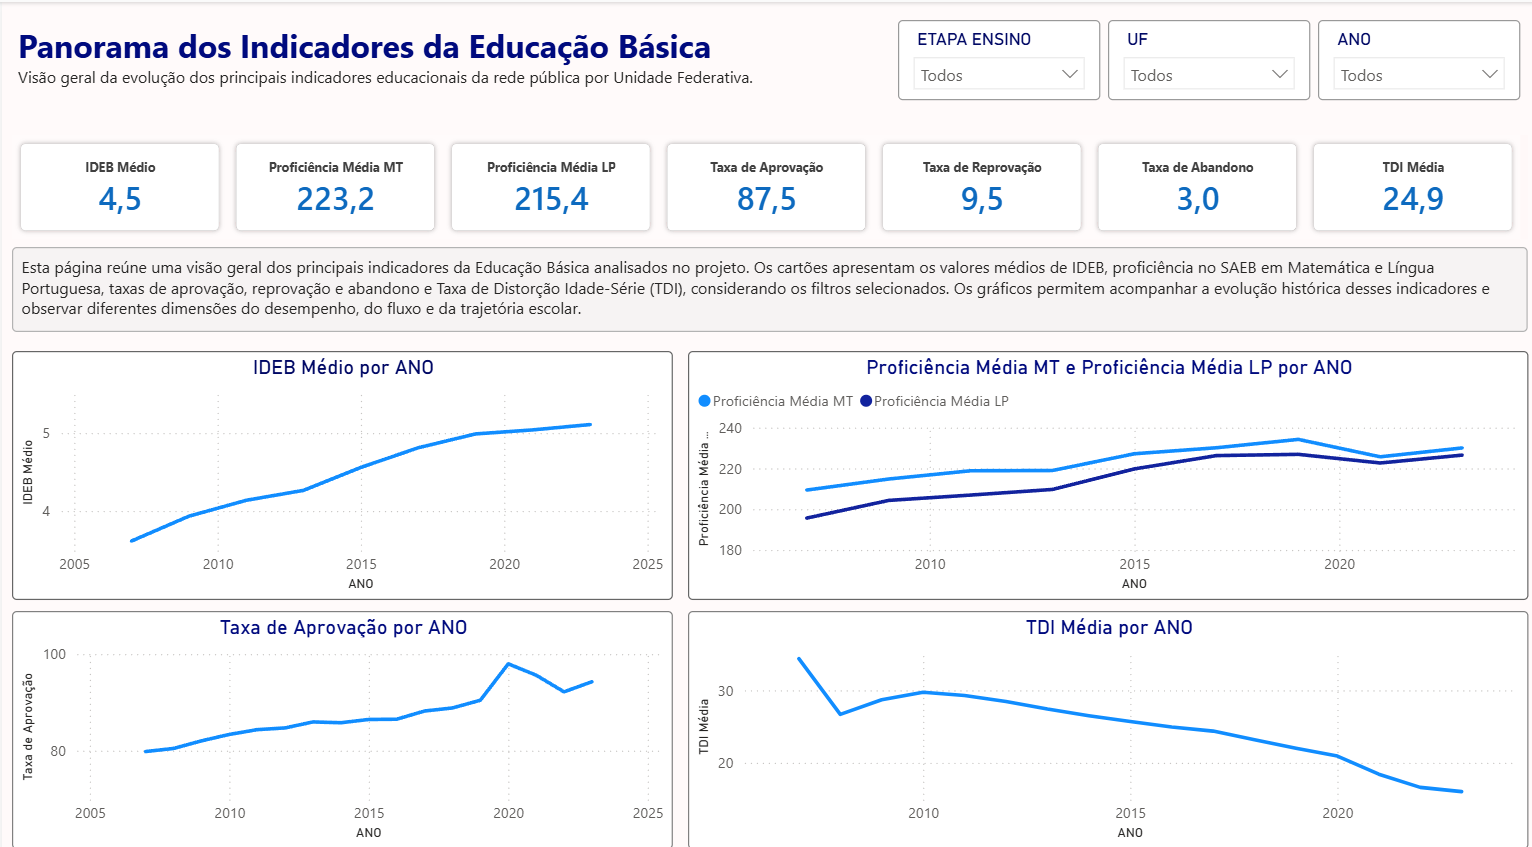
\includegraphics[width=0.98\textwidth]{figs/dashboard-panorama.png}
  \caption{Panorama dos indicadores da Educação Básica.}
  \label{fig:dashboard-panorama}
\end{figure}

\section{Desempenho educacional por Unidade Federativa}

A segunda página compara IDEB, SAEB Matemática, TDI e SAEB Língua Portuguesa entre Unidades Federativas em um ano de avaliação disponível. Na captura da Figura~\ref{fig:dashboard-uf}, o ano selecionado é 2007 e a etapa está em \textit{Todos}.

Nesse recorte, Paraná, Santa Catarina e São Paulo aparecem com IDEB médio de 4,4 entre as barras visíveis. No SAEB, o Distrito Federal aparece no topo visível tanto em Matemática, com 228,4 pontos, quanto em Língua Portuguesa, com 213,0 pontos. Para TDI, Pará e Alagoas aparecem entre os maiores valores visíveis, com 50,1 e 49,9, respectivamente. Esses exemplos evidenciam que a posição de uma UF depende do indicador analisado e que desempenho, fluxo e atraso escolar não formam uma única dimensão.

A página utiliza rankings separados para evitar transformar indicadores de escalas e significados distintos em uma medida única. Diferenças territoriais de desempenho também podem coexistir com condições sociais e educacionais distintas. Em um recorte específico do SAEB 2023 para o 5º ano de escolas públicas do Rio Grande do Norte, \citeonline{de2026desigualdades} identificaram diferenças significativas de proficiência entre escolas urbanas e rurais e ressaltaram sua coexistência com características territoriais e socioeconômicas. Embora se trate de outro recorte analítico, o estudo reforça a necessidade de contextualizar a leitura dos rankings.

\begin{figure}[H]
  \centering
  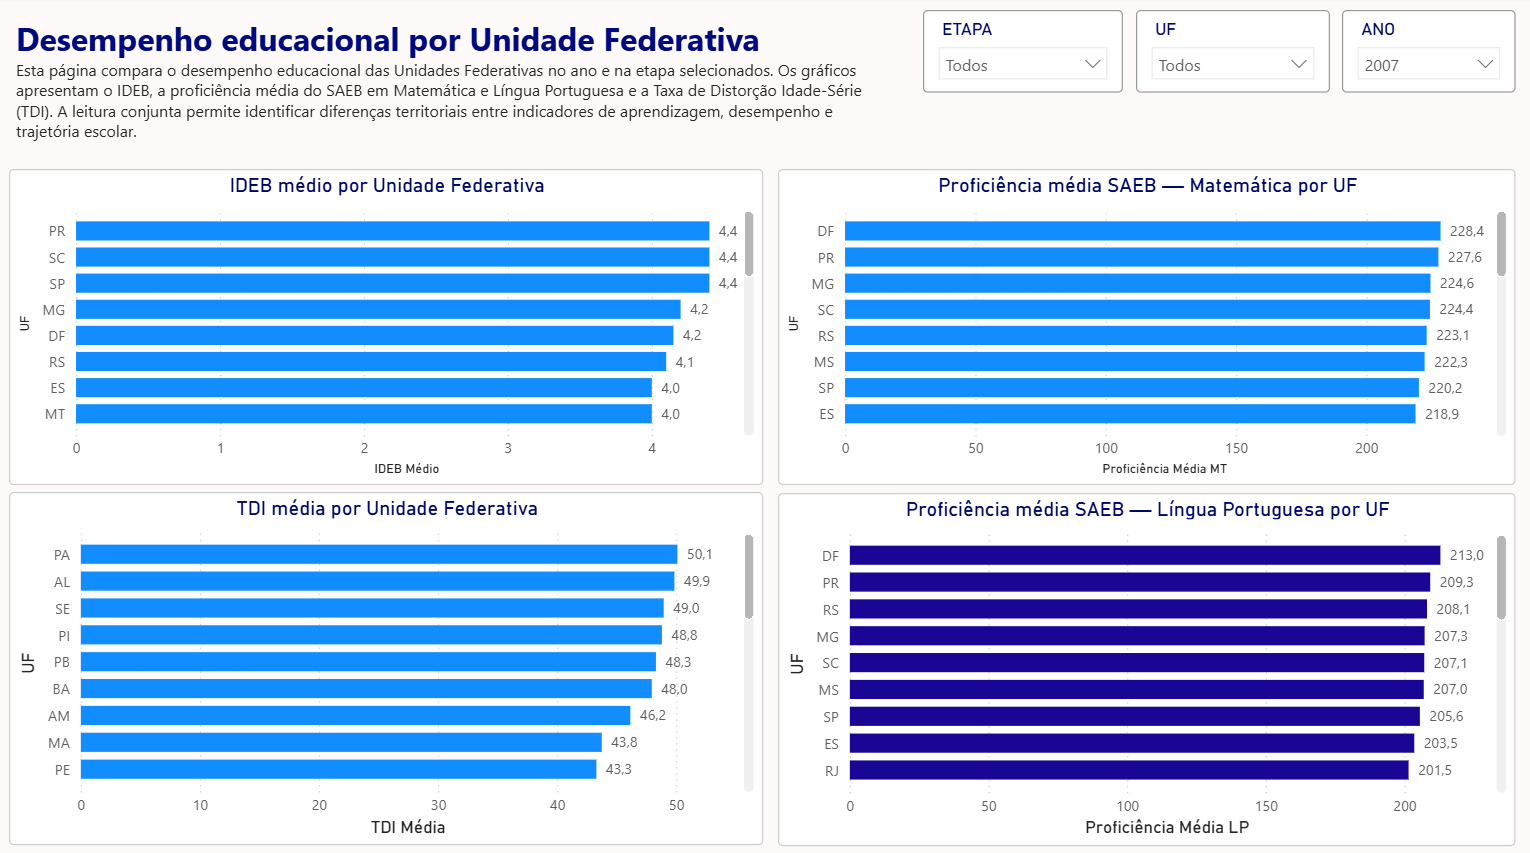
\includegraphics[width=0.98\textwidth]{figs/dashboard-ideb-saeb.png}
  \caption{Desempenho educacional por Unidade Federativa no recorte exibido no dashboard.}
  \label{fig:dashboard-uf}
\end{figure}

\section{Aprendizagem e fluxo escolar}

A página de aprendizagem e fluxo escolar combina duas formas de leitura. Na parte superior, são exibidas séries históricas de Aprovação, Reprovação, Abandono e TDI. Na parte inferior, cada ponto representa uma UF no ano selecionado, relacionando Taxa de Aprovação com IDEB e com proficiência média do SAEB.

Na Figura~\ref{fig:dashboard-aprendizagem-fluxo}, os gráficos históricos mostram aumento da aprovação ao longo do período e redução de TDI, reprovação e abandono em diferentes intensidades. Os gráficos de dispersão, por sua vez, permitem observar associação descritiva entre níveis mais elevados de aprovação e valores mais altos de IDEB ou proficiência em parte das UFs.

O IDEB combina informações de desempenho em avaliações com dados de fluxo escolar em sua composição \cite{inep2024ideb}, o que torna esperada alguma proximidade entre aprovação e IDEB. \citeonline{dias2026avaliaccao} ressaltam que, embora o IDEB seja um instrumento relevante de diagnóstico e planejamento, sua condição de indicador sintético exige interpretação contextualizada, evitando reduzir a complexidade educacional a uma única medida. A dispersão entre aprovação e proficiência do SAEB, por sua vez, deve ser lida apenas como associação descritiva.

\begin{figure}[H]
  \centering
  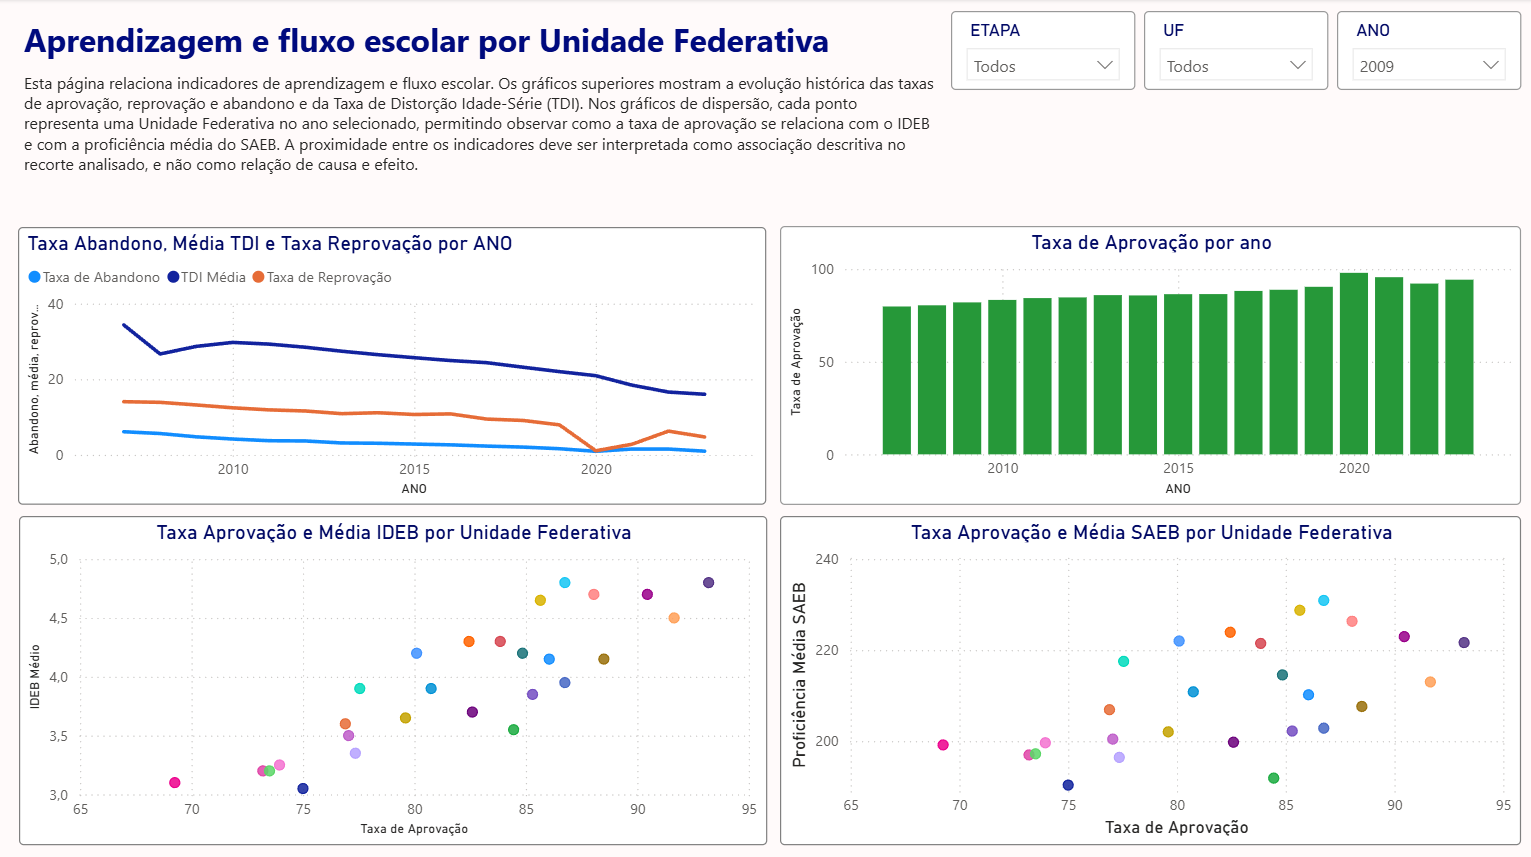
\includegraphics[width=0.98\textwidth]{figs/dashboard-aprendizagem-fluxo.png}
  \caption{Aprendizagem e fluxo escolar por Unidade Federativa.}
  \label{fig:dashboard-aprendizagem-fluxo}
\end{figure}

\section{Variação dos indicadores por Unidade Federativa}

As medidas de variação comparam o último e o primeiro ano com dado disponível dentro do intervalo selecionado para cada indicador. Isso evita supor observações anuais onde a fonte é bienal. As unidades também diferem: IDEB é expresso em pontos do índice; Aprovação, em pontos percentuais; e SAEB, em pontos de proficiência.

Na Figura~\ref{fig:dashboard-variacao}, o intervalo selecionado é 2007--2023. Entre as barras visíveis, Ceará apresenta a maior variação de IDEB, com 2,6 pontos, e também a maior variação de proficiência em Língua Portuguesa, com 60 pontos, além de 51 pontos em Matemática. Na Taxa de Aprovação, Alagoas aparece com aumento de 27 pontos percentuais. Esses valores descrevem diferença entre extremos observados no período e não uma taxa de crescimento relativa.

As diferenças territoriais reforçam que a evolução não ocorre de forma uniforme entre as UFs.

\begin{figure}[H]
  \centering
  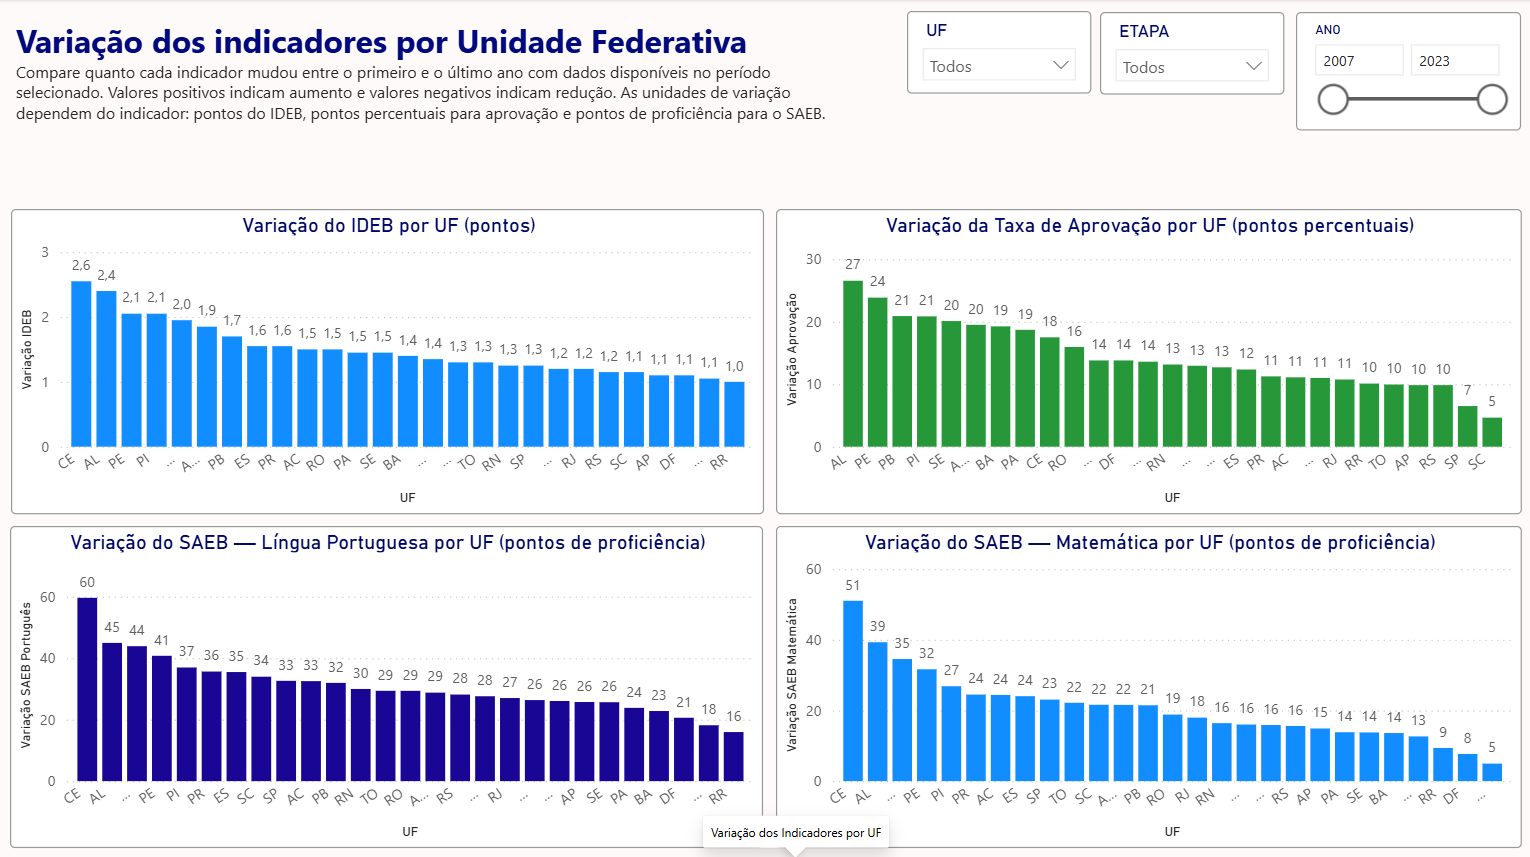
\includegraphics[width=0.98\textwidth]{figs/dashboard-variacao.png}
  \caption{Variação dos indicadores por Unidade Federativa no intervalo 2007--2023.}
  \label{fig:dashboard-variacao}
\end{figure}

\section{Análise da Taxa de Distorção Idade-Série}

A Figura~\ref{fig:dashboard-tdi} apresenta a TDI em quatro perspectivas: evolução anual, média por UF, média por etapa de ensino e variação por UF. No intervalo 2007--2023 mostrado no painel, a TDI média é 24,9 e a Variação TDI é -18,3 pontos percentuais.

A evolução temporal passa de 34,4 no início da série exibida para 16,0 em 2023. Por etapa, os Anos Finais apresentam TDI média de 32,3, enquanto os Anos Iniciais apresentam 17,5. No ranking de médias por UF, Sergipe aparece com 37,2 e São Paulo com 8,6 nos extremos visíveis do painel. A variação territorial é negativa para todas as barras exibidas, indicando redução da distorção no intervalo considerado, embora em magnitudes diferentes entre as UFs.

A redução é um resultado favorável sob a interpretação do indicador, pois a TDI expressa a proporção de estudantes em situação de distorção entre idade e série \cite{inep2026tdi}; portanto, valores menores indicam menor incidência dessa condição no recorte analisado. Contudo, a permanência de médias elevadas em determinadas UFs e a diferença entre etapas mostram que o problema não desaparece de forma homogênea. \citeonline{leal2025distorccao} discute a distorção idade-série como um fenômeno associado a fatores pedagógicos, sociais e estruturais, entre eles repetência e vulnerabilidade socioeconômica, aspectos que não são modelados pelo dashboard.

\begin{figure}[H]
  \centering
  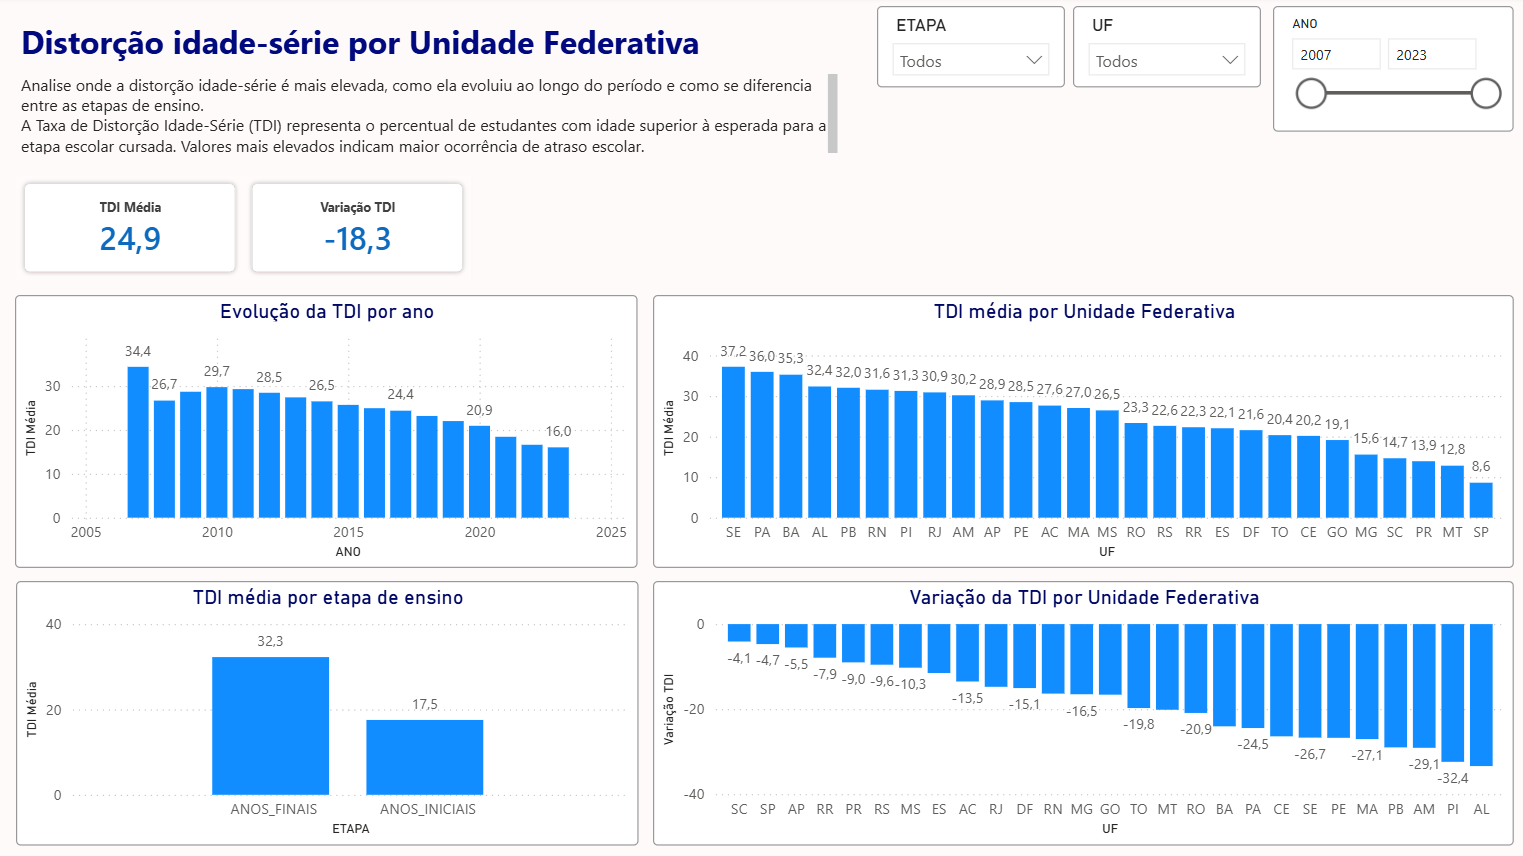
\includegraphics[width=0.98\textwidth]{figs/dashboard-tdi.png}
  \caption{Distorção idade-série por Unidade Federativa e etapa de ensino.}
  \label{fig:dashboard-tdi}
\end{figure}

\section{Resultados da PND 2025}

A PND é analisada separadamente das séries históricas. A população analítica contém 759.140 registros. A classificação utilizada no projeto é baseada em \texttt{NT\_OBJ} e nos pontos de corte documentados para a PND \cite{inep2025notatecnica44,inep2026notatecnica1}. Aplicando essa regra à população analítica, obtiveram-se 265.932 não proficientes, 304.638 participantes no Padrão 1 e 188.570 no Padrão 2. A soma dos padrões 1 e 2 corresponde a 493.208 proficientes, equivalentes a 64,97\% da população analítica.

Na Figura~\ref{fig:dashboard-pnd}, os cartões arredondam esse resultado para 759 mil participantes e 65,0\% de proficientes. A Nota Objetiva Média exibida é 57,5 e a Nota Geral Média é 57,3. Os gráficos complementam a leitura com percentual de proficientes por área, percentual de proficientes por UF, nota objetiva média por área e distribuição dos três padrões por UF.

A classificação deve ser interpretada nos termos dos pontos de corte aplicados à nota objetiva \cite{inep2025notatecnica44,inep2026notatecnica1}. Não se trata de aprovação ou reprovação e o limite de 50 pontos não representa simplesmente 50\% de acertos. A distribuição por UF e área também é descritiva da população analítica da prova. Como \texttt{UF\_PROVA} representa a Unidade Federativa de aplicação, diferenças territoriais não devem ser interpretadas automaticamente como características de residência dos participantes.

\begin{figure}[H]
  \centering
  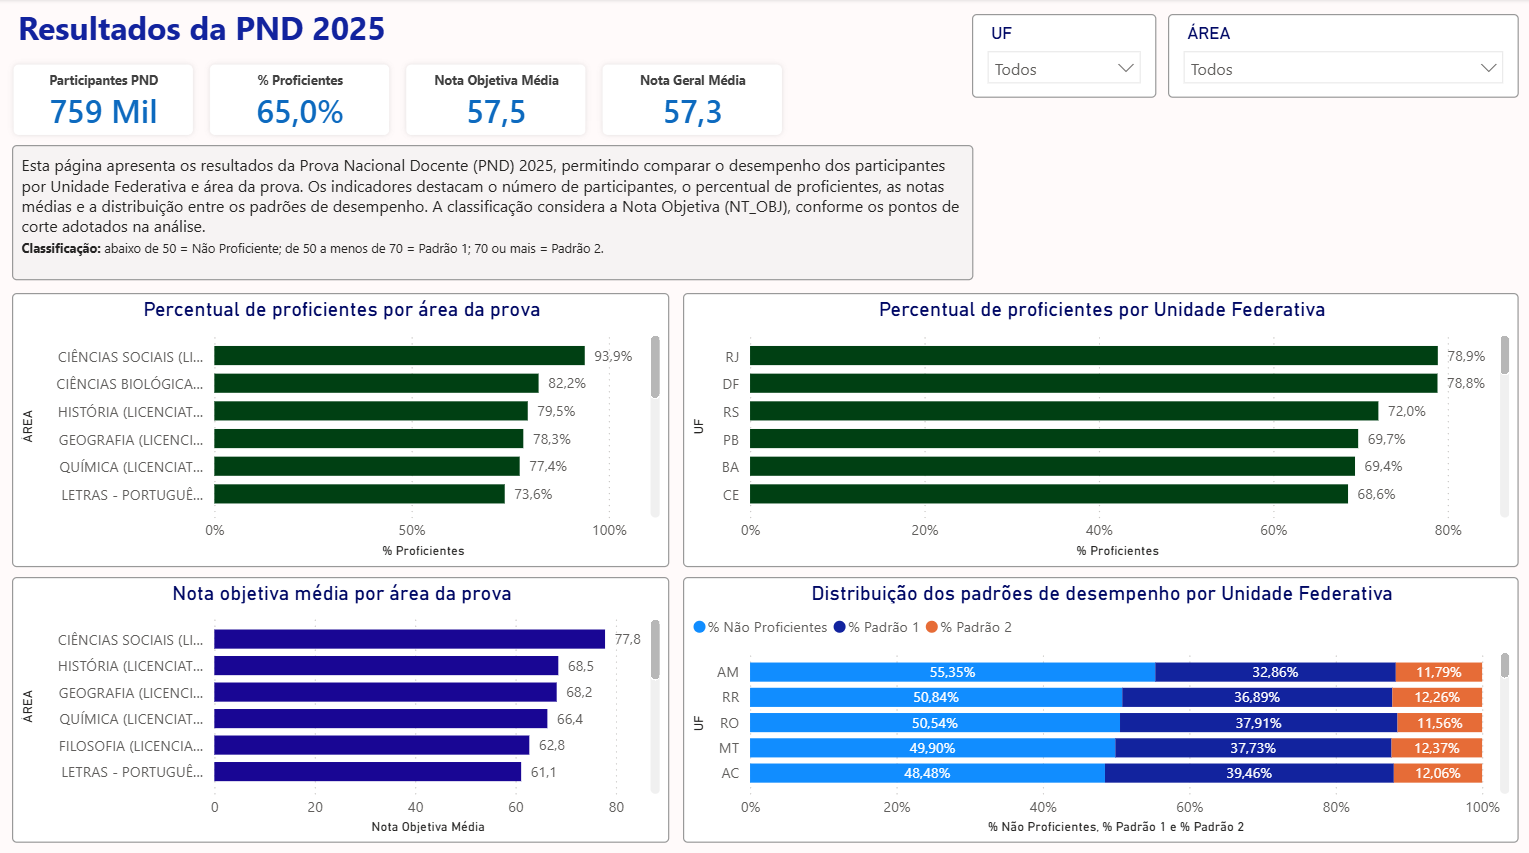
\includegraphics[width=0.98\textwidth]{figs/dashboard-pnd-medias.png}
  \caption{Resultados da Prova Nacional Docente de 2025.}
  \label{fig:dashboard-pnd}
\end{figure}

\section{Limitações observadas nos resultados}

Os resultados devem ser lidos em conjunto com as limitações metodológicas apresentadas na Seção~\ref{sec:limitacoes-metodologicas}. Em particular, as fontes diferem em periodicidade, nível de agregação e categorias históricas, enquanto a análise foi harmonizada principalmente por UF, rede pública e etapa de ensino.

Os cartões de média no Power BI calculam a média das linhas presentes no contexto de filtro. Quando todas as UFs estão selecionadas, esse valor não equivale automaticamente a um indicador nacional ponderado por matrícula ou por quantidade de participantes. Assim, os números gerais do dashboard devem ser interpretados como sínteses do modelo analítico construído, e não como substitutos de estatísticas nacionais oficiais produzidas com outros ponderadores.

Por fim, nenhuma associação visual apresentada neste capítulo deve ser interpretada como relação de causa e efeito. O projeto foi desenhado para integração, rastreabilidade e exploração descritiva dos dados; investigações causais exigiriam desenho metodológico, variáveis de controle e técnicas estatísticas específicas.
